\section{Introduction}
\label{1.0}


Recent developments in AI have triggered a new shift in deep learning models~\cite{kaplan2020scaling}. Future intelligent systems are expected to follow a dual paradigm: learn new knowledge, and remove specific knowledge. This capability is called Continual Learning and Unlearning (CLU) \cite{chatterjee2024unified,liu2022continual}, also termed continual adaptation. This capability becomes essential when data distributions shift over time, whether due to policy changes, task modifications, or market trends. Regardless of the underlying cause, the model's knowledge base must be updated accordingly. Fig~\ref{fig:1} illustrates CLU system as new data replaces unwanted data. This requires simultaneous systems for both learning and unlearning.

Since CLU combines Continual Learning (CL) and Machine Unlearning (MU), we establish each component's foundation. CL is the process of acquiring new knowledge~\cite{kirkpatrick2017overcoming,buzzega2020dark,caccia2021new,douillard2022dytox,cotogni2025exemplar,mohamed2023d3former} from unseen data while retaining performance on existing tasks, widely studied in machine learning. Application tasks include mixed-task scenarios, out of distribution tasks, among others. While CL focuses on knowledge acquisition, MU addresses selective knowledge removal, an emerging field~\cite{kurmanji2023towards,zhao2024continual,cha2024learning,fan2023salun,tarun2023fast}. Targets for unwanted knowledge removal include privacy-related data, regulatory removal by government orders such as General Data Protection Regulation (GDPR) and California Consumer Privacy Act (CCPA)~\cite{goldman2020introduction,data2018general}, and hate speech, among others.

\begin{figure}[!htbp]
    \centering
    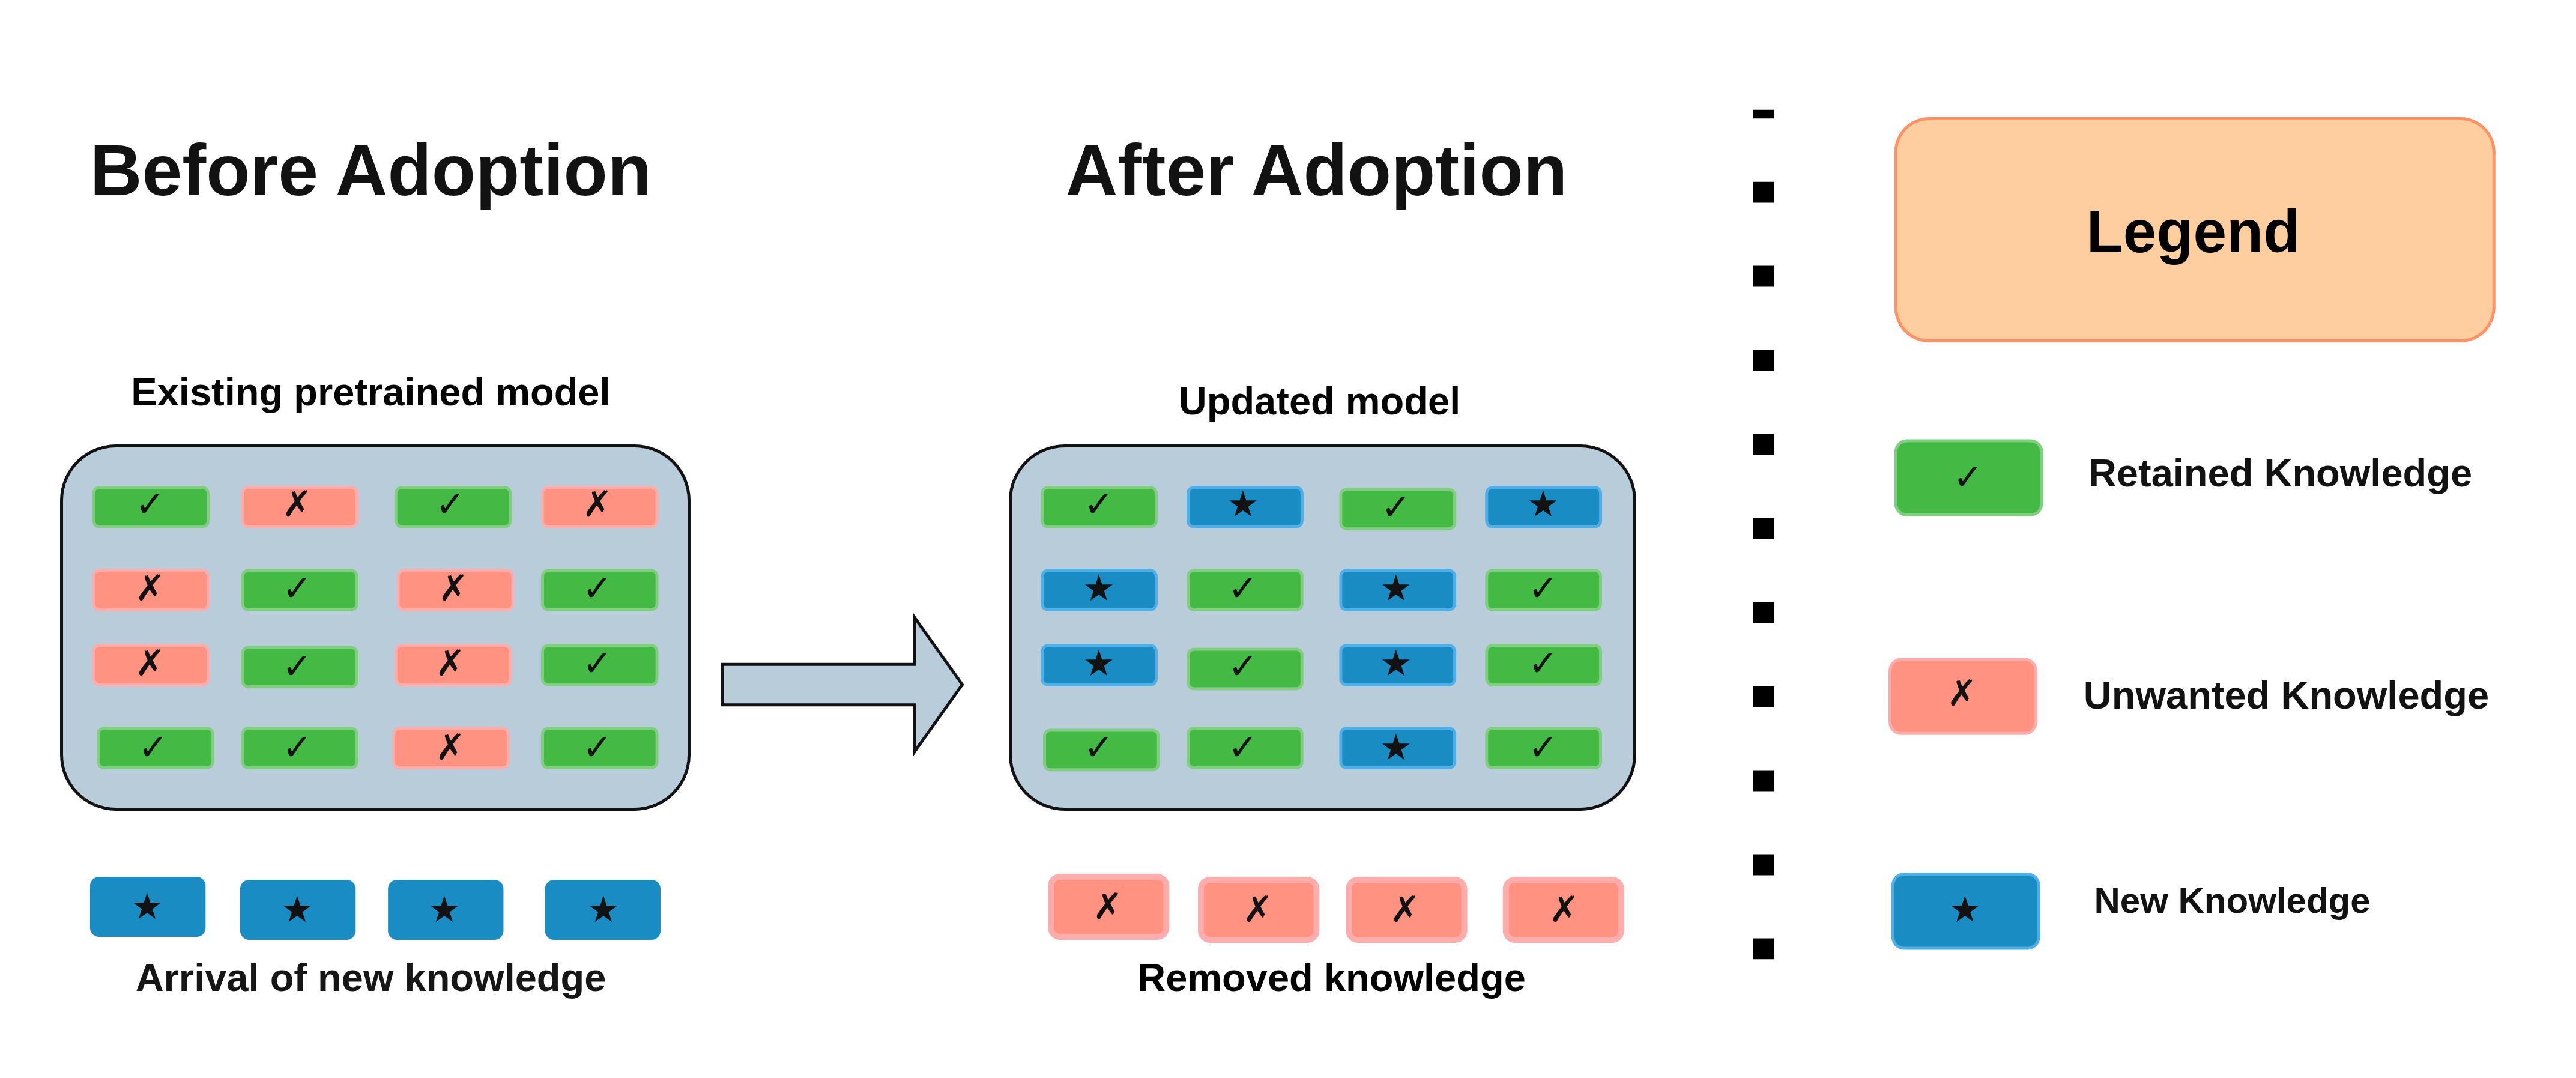
\includegraphics[width=0.75\textwidth]{images/overview.drawio.png}
    \caption{Overview of CLU. The CLU system removes unwanted knowledge (\textcolor{red}{red}), retains prior knowledge (\textcolor[HTML]{006400}{green}), and integrates new knowledge (\textcolor{blue}{blue}).}
    \label{fig:1}
\end{figure}


There is an intrinsic connection between MU and CL in which one adds knowledge and other removes knowledge, both retaining existing knowledge. Can we combine both for simultaneous learning and unlearning? Such a framework would enable access control, surveillance, personalized education, and content moderation. Can continual learning alone solve this? No-without removing unwanted knowledge over time, it accumulates and causes knowledge drift   degrading model performance and creating bias toward unwanted information, making unlearning essential.

Despite CLU's importance, a research gap exists due to maturity imbalance. CL is well-established, while Machine Unlearning remains developmental. This disparity leaves unified CLU frameworks largely unexplored. CLU applications demand parameter-efficient solutions. CLU systems continuously adapt as data arrives and require removal. Full retraining becomes computationally infeasible, making parameter-efficient approaches essential. However, combining CL and MU introduces knowledge leakage-repeated learning-unlearning cycles cause models to gradually lose foundational knowledge. Unlike catastrophic forgetting, knowledge leakage is a slow degradation of original capabilities across adaptation cycles; further analysis is provided in Section~\ref{8.2}. This challenge is critical because real-world systems face continuous requests: employees join and leave organizations, regulations evolve, and user preferences shift constantly. Such systems with minimal knowledge leakage would enable critical applications: language models, medical systems, recommendation engines, and autonomous vehicles. Face recognition presents the most urgent CLU need due to privacy challenges.


Face recognition systems are critical CLU applications as personnel frequently join and leave organizations. Since facial data is highly sensitive private information, protecting it from misuse through model inversion techniques~\cite{fredrikson2015model,zhu2019deep,zhang2020secret} becomes essential to safeguard privacy rights mandated by GDPR and CCPA~\cite{goldman2020introduction,data2018general}. Face recognition thus provides a natural testbed for CLU applications, presenting an urgent challenge that demands immediate attention given the escalating privacy threats and regulatory requirements. Designing such an ideal CLU system presents three core challenges. First, achieving continual learning while avoiding catastrophic forgetting. Second, implementing selective machine unlearning. Finally, maintaining knowledge stability and minimizing knowledge leakage across repeated cycles. 

To address these challenges, we propose Bi-Directional LoRA (BID-LoRA), a parameter-efficient solution to CLU problems that minimizes knowledge leakage. BID-LoRA leverages LoRA's inherent parameter efficiency, fine-tuning only attention layers in transformer blocks and classification heads~\cite{houlsby2019parameter,hu2022lora,li2021prefix,geva2020transformer} as fine-tuning fewer parameters has been shown effective~\cite{mallya2018packnet,mallya2018piggyback,wang2022learning,zhang2022continual} in knowledge manipulation. To reduce catastrophic forgetting~\cite{kirkpatrick2017overcoming} and minimize knowledge leakage, we employ the replay mechanism. This approach is similar to performing minimally invasive surgery on a model rather than major surgery. BID-LoRA is simple, parameter-efficient, data-efficient, and suitable for large models. We conduct extensive experiments across classification and face recognition tasks, demonstrating broad applicability. Our contributions are summarized as follows:
\label{contributions}
\begin{itemize}
    \item We formally define the Continual Learning-Unlearning (CLU) problem and demonstrate that naively combining existing CL and MU approaches leads to significant knowledge leakage, where foundational knowledge degrades across repeated adaptation cycles.
    
    \item We propose BID-LoRA, a parameter-efficient framework featuring three-pathway separation that isolates retained, forgotten, and newly learned knowledge. This architecture prevents interference between competing objectives while updating only $\approx$5\% of model parameters.
    
    \item We introduce escape unlearning, which computes optimal embedding locations that are maximally distant from retained class centroids, pushing forget-class representations to positions that are both hard to recover and non-interfering with retained knowledge.
    
    \item We establish the first generalizable CLU benchmark through comprehensive experiments on CIFAR-100 and CASIA-Face100, employing a novel sliding window evaluation protocol with progressive 10-class forget-retain-learn cycles that systematically tests long-term adaptation stability.
    
    \item We demonstrate BID-LoRA's practical applicability to face recognition and identity management systems, where privacy-driven unlearning (e.g., GDPR compliance) must coexist with incremental enrollment of new users.
\end{itemize}